\documentclass[11pt]{amsart}
\usepackage{geometry}                % See geometry.pdf to learn the layout options. There are lots.
\geometry{a4paper}                   % ... or a4paper or a5paper or ...
%\geometry{landscape}                % Activate for for rotated page geometry
\usepackage[parfill]{parskip}    % Activate to begin paragraphs with an empty line rather than an indent
\usepackage{enumitem}
\usepackage{graphicx}
\usepackage{amssymb}
\usepackage{amsmath}
\usepackage{cancel}
\usepackage{epstopdf}
\DeclareGraphicsRule{.tif}{png}{.png}{`convert #1 `dirname #1`/`basename #1 .tif`.png}
\usepackage{breqn}
\usepackage{float}
\usepackage{breqn}

\title{Econ 210C Problem Set \# 4}
\author{Minki Kim}
%\date{}                                           % Activate to display a given date or no date

\begin{document}




\maketitle

\section{Labor supply problem}
\begin{enumerate}[label=(\alph*)]
	\item individuals with time-separable utility solve the following maximization problem: 
	\begin{equation*}
	\mathcal{L} = \sum_{t=0}^{\infty} \beta^t \bigg( \log C_t + \log (1-L_t) \bigg) + \lambda \sum_{t=0}^{\infty} \beta^t \left( C_t - w_t L_t \right)
	\end{equation*}
	Since the future wage schedule is known in advance, the problem is translated into the following form:
	\item
\end{enumerate}
\section{Demand shock}
\begin{enumerate}[label=(\alph*)]
	\item 
	\item
	\item
	\item
	\item
\end{enumerate}
\section{Business cycle and external returns to scale}
\begin{enumerate}[label=(\alph*)]
	\item 
	\item
	\item
	\item
	\item
\end{enumerate}
\section{Problems from Romer}
\subsection{Problem 6.10}
\begin{enumerate}[label=(\alph*)]
	\item Using the given three equations, it is easy to get the closed form solution for $p, p^{*}$, and $y$. 
	\begin{align*}
	p & = \frac{f \phi m'}{1 - f + f\phi} \\
	p^{*} & = \frac{\phi m'}{1 - f + f\phi} \\
	y & = \frac{m' (1-f)}{1 - f + f\phi}
	\end{align*}
	\item The following figure summarizes the results
	\begin{figure}[H]
		\centering
		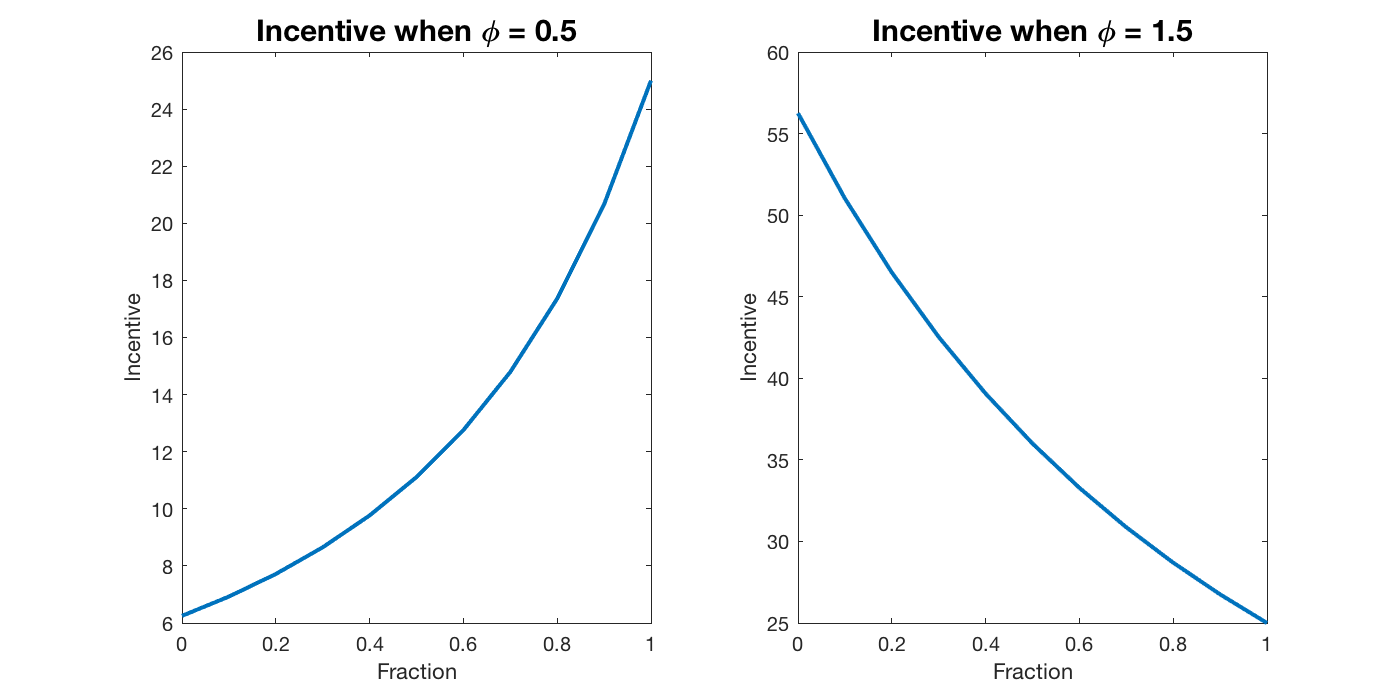
\includegraphics[width=0.85\textwidth]{611b}
		\caption{A firm's incentive to adjust its price}
	\end{figure}
	\item Whether a firm adjusts its price or not depends on the size of the menu cost, $Z$. Suppose $\phi <1$. To be written...
\end{enumerate}
\subsection{Problem 6.11}
\begin{enumerate}[label = (\alph*)]
	\item If the firm does not adjust its price and stays at $r^{*}(y_0)$ level, its profit is $\pi \left( y_1, r^{*}(y_0)  \right)$. On the other hand, if the firm choose to adjust its price to the optimal level for $y_1$, its profit is $\pi \left( y_1, r^{*}(y_1)  \right)$ The difference between these two is a potential gain from adjusting the price, so can be interpreted as the incentive to adjust its price. 
	\item Second-order Taylor approximation of $G = \pi \left( y_1, r^{*}(y_1)  \right) - \pi \left( y_1, r^{*}(y_0)  \right)$ is: 
	
	\begin{align*}
	G &= \pi \left( y_1, r^{*}(y_1)  \right) - \pi \left( y_1, r^{*}(y_0)  \right) \\
	 & \simeq 
	\end{align*}
	\item 
\end{enumerate}
\subsection{Problem 6.12}

\end{document}
